\documentclass[a4paper, 12pt, twoside]{book}
	\PassOptionsToPackage{table}{xcolor}
	\usepackage[export]{adjustbox}
	\usepackage[english,ngerman]{babel}
	\usepackage{amsmath, url}
	\usepackage[utf8]{inputenc}
	\usepackage[dvipsnames]{xcolor}
	\usepackage[T1]{fontenc}
	\usepackage{import}
	\usepackage{graphicx}
	\usepackage{subcaption}
	\usepackage{verbatim}
	\usepackage{float}
	\usepackage[headheight=12pt]{geometry}
	\usepackage{fancyhdr}
	

	%  Bibliographie
\usepackage{bibgerm} % Umlaute in BibTeX
%\usepackage[style=authortitle-icomp]{biblatex}
\bibliographystyle{abbrv} 
\usepackage[babel,german=guillemets]{csquotes}

	

	\pagestyle{fancy}
	\fancyhf{}
	\fancyhead[LE,RO]{Baran Avinc}
	\fancyhead[RE,LO]{Masterarbeit}
	\fancyfoot[LE,RO]{\vspace{0.05cm}\thepage}
	%\fancyfoot[RE,LO]{\vspace{0.05cm}
\includegraphics[width=0.1\textwidth]{Bilder/TU-Berlin-Logo.pdf}}
	\renewcommand{\headrulewidth}{1pt}
	\renewcommand{\headrule}{\hbox to\headwidth{\color{RoyalPurple}\leaders\hrule height 				\headrulewidth\hfill}}
	\renewcommand{\footrulewidth}{1pt}
	\renewcommand{\footrule}{\hbox to\headwidth{\color{RoyalPurple}\leaders\hrule height \footrulewidth\hfill}}
	\pagestyle{fancy}


	


  	%
\includegraphics[width=0.1\textwidth]{Bilder/TU-Berlin-Logo.pdf}

	





\begin{document}
	
\begin{titlepage}
		\pagestyle{fancy}
		\centering\textbf{\large Masterarbeit zum Thema}\\
		\vspace{3cm} 
		\noindent{\color{RoyalPurple}\rule{\textwidth}{1pt}} \\
		\vspace{0.5cm} 
		\centering\textbf{\large Untersuchung der optischen Polarisation und internen Quanteneffizienz von AlGaN Quantenfilmen mittels temperatur- und leistungsabhängiger Photolumineszenzspektroskopie} \\
		\vspace{0.25cm} 
		\noindent{\color{RoyalPurple}\rule{\textwidth}{1pt}} \\
		\vspace{3cm}
		\centering Baran Avinc \\
		\vspace{3cm}
		\centering Institut für Festkörperphysik
		\vspace{\fill} \\
		\raggedleft{
\includegraphics[width=0.2\textwidth]{Bilder/TU-Berlin-Logo.pdf}}
\end{titlepage}



	\tableofcontents\thispagestyle{fancy}
	
\chapter{Einleitung}
\thispagestyle{fancy}

\begin{quote}
In the spirit of Alfred Nobel the Prize rewards an invention of greatest benefit to mankind; using blue LEDs, white Light can be created in a new way.\end{quote}
Dieser Satz den die Schwedische Akademie der Künste nach der Vergabe des Nobelpreises an die Entwicklung der blauen LED(kurz, light emitting diode) im Jahr 2014 an die Presse veröffentlichte, fasst treffend zusammen, wie hoch die Bedeutung der auf Halbleiterkristallen basierenden optischen Bauelemente ist.
LEDs nehmen einen fundamentalen und immer bedeutender werdenden Teil unseres alltäglichen Lebens ein. Ausgezeichnet durch ihre hervorragende Effizienz, konkurrenzlosen Lebensdauer und geringen Dimension übernimmt sie durch eine immer höher werdenden Lichtausbeute zusehends neue Anwendungsbereiche. 
%Seit jeher etabliert in den Bereichen der optischen Datenübertragung und Leuchtanzeige schreiten immer mehr andere Wellenlängenbereiche in den Fokus der weltweiten Forschung. 
Insbesondere auf Gallium Nitrid (GaN) basierende Halbleitermaterialien haben einen bahnbrechenden Weg hingelegt, der zur Entwicklung von hoch effizienten und leuchtstarken blauen LEDs führte.




	\chapter{Grundlagen}
\thispagestyle{fancy}

\section{Bandstruktur von Gruppe-III Nitriden}
\begin{figure}[!htb]
    \centering
    \begin{minipage}[t]{\linewidth}
        \centering
        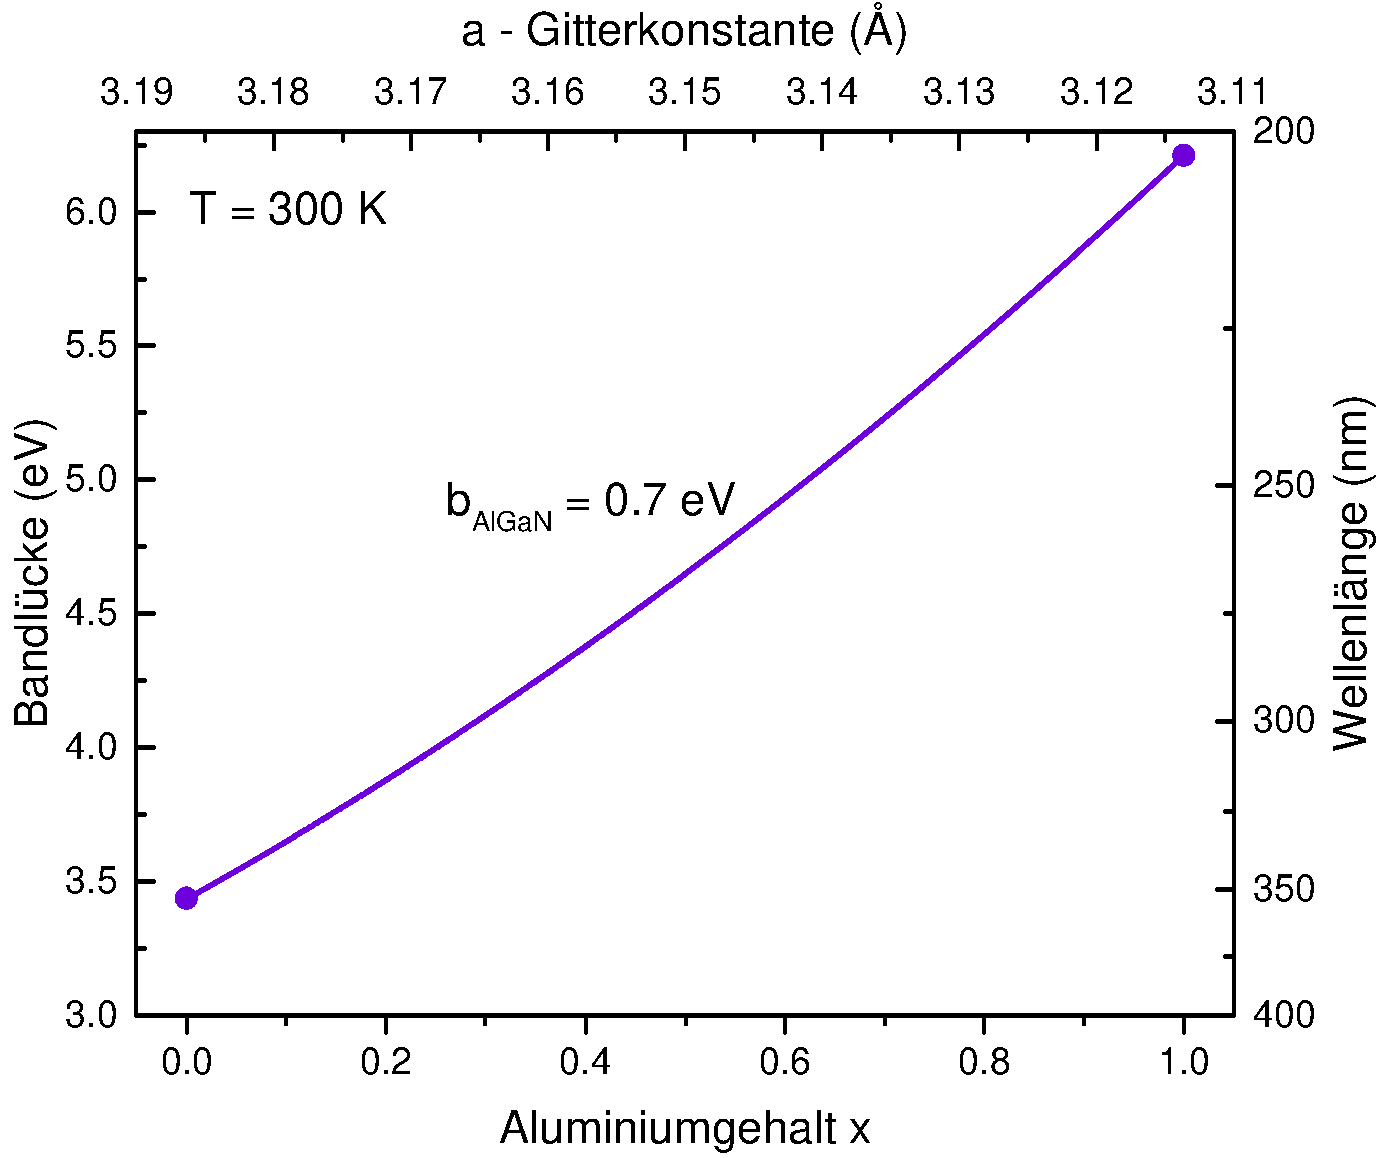
\includegraphics[width=0.5\linewidth]{Bilder/bandluecke.pdf}
        \caption{Die Bandlücke von $Al_{x}Ga_{1-x}N$ variiert mit dem Aluminiumgehalt x zwischen den Bandlücken von AlN ($E_{g}(T = 300 K) = 6,213 \thinspace eV$) und GaN ($E_{g}(T = 300 K) = 3,437 \thinspace  eV$) ~\cite{pipr}. Die Abweichung von der Linearität beschreibt der Bowing-Parameter $b_{AlGaN} = 0,7 \thinspace eV$.} 
        \label{fig:wurtz}
    \end{minipage}% <- sonst wird hier ein Leerzeichen eingefügt
\end{figure}
\noindent
Der Schwerpunkt dieser Arbeit liegt auf dem AlGaN-Materialsystem mit hohen Al-Konzentrationen. Das Mischverhältnis bestimmt hierbei die Bandlückenenergie des Verbindungshalbleiters. Durch die unterschiedlichen Bandlückenenergien von Aluminium mit $6,03 \thinspace eV$\cite{fenaln} und GaN mit $3,4 \thinspace eV$ \cite{pipr} eignet sich AlGaN besonders für die Emission im Wellenlängenbereich von UV-A bis UV-C. 
Die Bandlückenenergie von AlGaN lässt sich durch Interpolation der binären Energien von GaN und AlN in Abhängigkeit des Kompositionsverhältnisses x berechnen, wobei ein zusätzlicher Bowing-Parameter für die nichtlineare Abweichung hinzugefügt wird. 
%
\begin{equation}
    E_{Al_{x}Ga{1-x}N} = E_{AlN} \cdot x + E_{GaN} \cdot (1-x) - b_{AlGaN} \cdot x \cdot (1-x) 
\end{equation}
%
Die Gruppe um Lee et al. gibt nach Auswertung der in der Literatur vorkommenden unterschiedlichen Bowing-Parameter für $Al_{x}Ga_{1-x}N$ einen Wert von $b_{AlGaN} = 0,62\thinspace(\pm \thinspace 0,45)\thinspace eV$ an und ergänzt, dass hohe Wachstumstemperaturen zu großen Bowing-Parametern führen \cite{doi:10.1063/1.123339}.
Vurgaftman et al. empfehlen unter Berücksichtigung weiterer Veröffentlichungen für $b_{AlGaN} =  0,7 \thinspace eV$.



\section{Wurtzitstruktur}

\begin{figure}[!htb]
    \centering
    \begin{minipage}[t]{\linewidth}
        \centering
        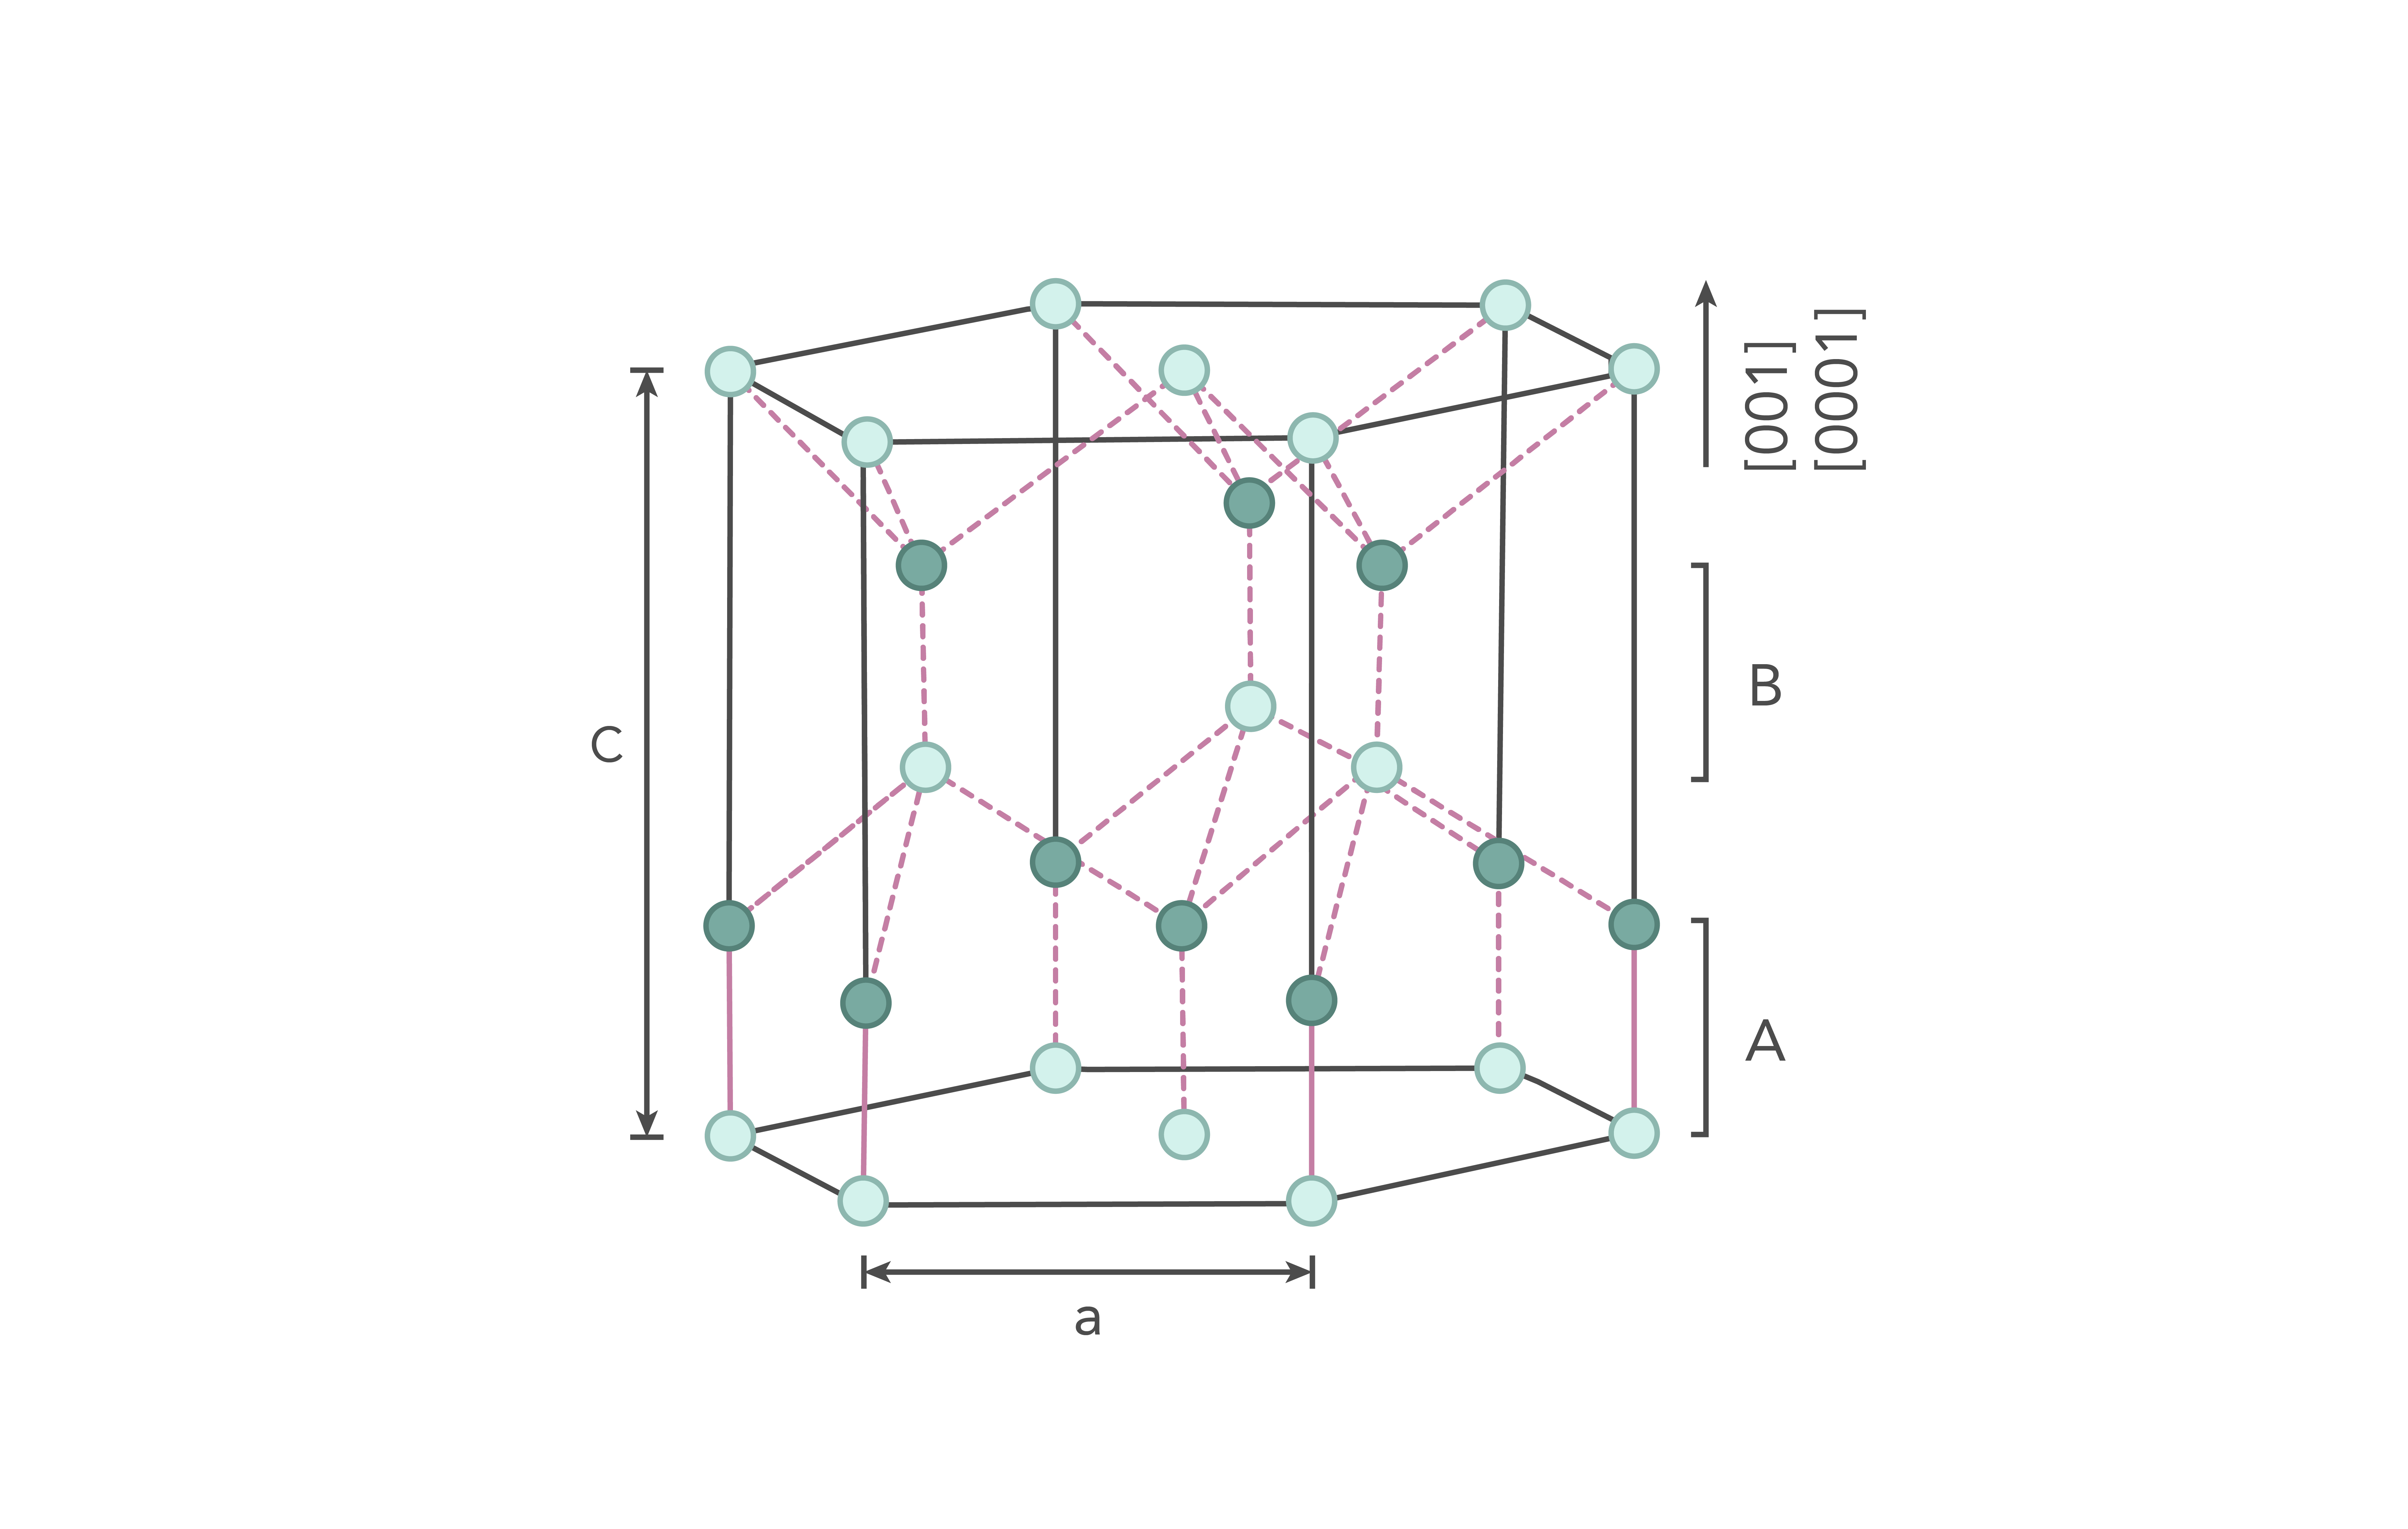
\includegraphics[width=0.8\linewidth]{Bilder/Wurtzite.png}
    \end{minipage}% <- sonst wird hier ein Leerzeichen eingefügt
     \caption{Einheitzelle der hexagonalen Wurtzitstruktur. Die schwarzen Kreise stellen die Position der Stickstoffatome im Gitter dar. Die Gitterposition der Gruppe-III-Metallatome sind als graue Kreise dargestellt. A und B bezeichnen die Stapelebenen.}
        \label{fig:wurtz}
\end{figure}
\noindent
Die wichtige Gruppe der III-Nitridhalbleiter setzt sich aus den Metallen
der dritten Hauptgruppe Aluminium (Al), Gallium (Ga) und Indium (In) zusammen.
Diese kristallisieren, wie in Abbildung \ref{fig:wurtz} zu sehen, bevorzugt in der hexagonalen Wurtzitstruktur. Anschaulich bedeutet dies, dass ausgehend von der hexagonal dichtesten Kugelpackung in Doppellagen, die Gruppe-III-Metalle und Stickstoff (N) sich entlang der c-Achse in der Abfolge A-B-A-B anordnen \cite{buchc}. Die Einheitszelle wird durch Gitterparameter $a$ und $c$ bestimmt. Die Gitterkonstanten zeigen eine lineare Abhängigkeit vom Konzentrationsverhältnis x und können mit dem Vegard'schen Gesetz berechnet werden.
%
\begin{align}
\begin{split}
    a_{Al_{x}Ga{1-x}N} &= a_{AlN} \cdot x + A_{GaN} \cdot (1-x)  ,
    \\
    c_{Al_{x}Ga{1-x}N} &= c_{AlN} \cdot x + A_{GaN} \cdot (1-x) 
\end{split}
\end{align}
%
Die Tabelle \ref{table:tab1} zeigt die typischen Gitterkonstanten.
\begin{figure}[H]
\centering
\begin{tabular}{|c|c|c|c|}
\hline
\multicolumn{1}{|l|}{Gitterkonstante} & AlN & GaN & Saphir \\ \hline \hline
a & 3,112 & 3,192 & 4,758 \\ \hline
c & 4,980 & 5,196 & 12,99 \\ \hline
\end{tabular}
\caption{Übersicht der Gitterkonstanten der binären Halbleiter AlN, GaN und $Al_{2}O_{3}$ (Saphir). ~\cite{pohl} }
\label{table:tab1}
\end{figure}

\section{Polarisationsfeld und QCSE in III/V Halbleitern}

Aufgrund der fehlenden Inversionssymmetrie und stark unterschiedlichen Elektronegativitäten des Stickstoffs und der entsprechenden Gruppe III-Metalle bilden sich Polarisationsfelder aus, die entlang der auf der Basalebende stehenden c-Achse verlaufen. Hier unterscheidet man zwischen zwei Arten von Polarisationsfeldern, die spontane Polarisation $ \vec{P}^{sp} $ und die piezoelektrische Polarisation $ \vec{P}^{pz} $. Die spontane Polarisation entsteht durch Dipolmomente im Kristall, die sich aufgrund von ungleichen Bindungslängen nicht komplett aufheben. Ursprung der 
Dipolmomente im AlGaN sind die unterschiedlichen Elektronegativitäten zwischen den Gruppe III-V Elementen. Bedingt durch die angestrebte Minimierung der Gesamtenergie kommt es zur Abweichung vom idealen Tetraederwinkel von $109,5^{\circ}$~\cite{ambacher2002}.
%
\begin{figure}[htb]
    \centering
    \begin{minipage}[t]{1.0\linewidth}
        \centering
        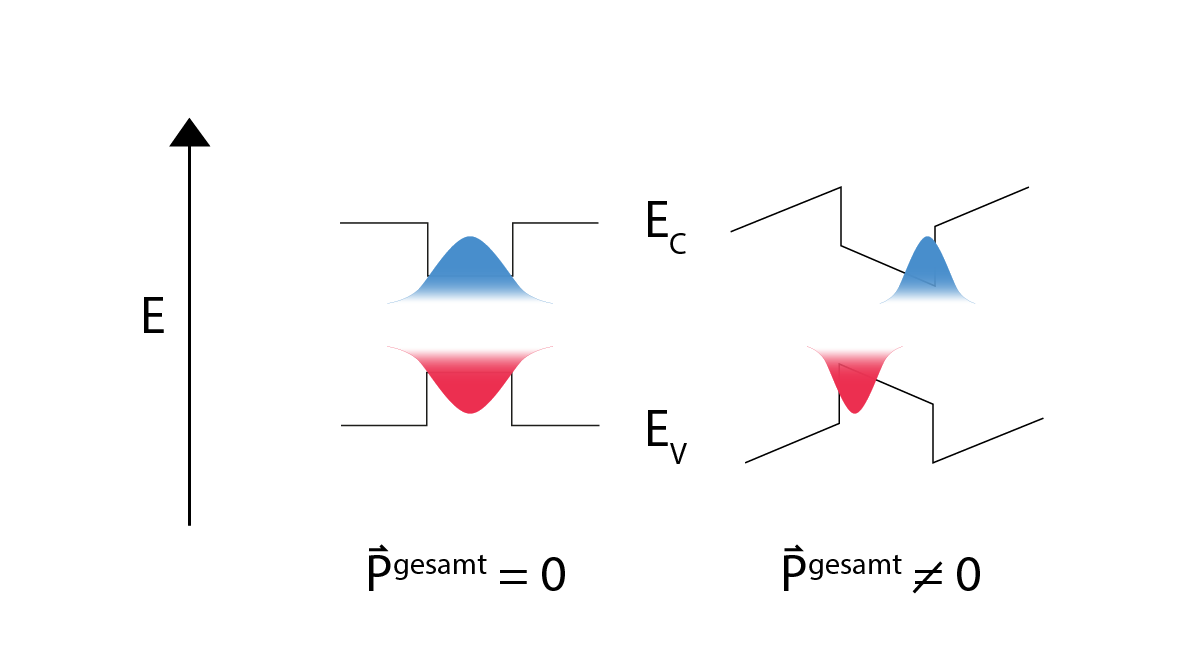
\includegraphics[width=0.7\linewidth]{Bilder/QCSE.png}
    \end{minipage}% <- sonst wird hier ein Leerzeichen eingefügt
    \caption{Einfluss der spontanen und piezolektrischen Polarisation auf Valenz- und Leitungsband einer Quantenfilm-Heterostruktur. Die Aufenthaltswahrscheinlichkeiten von Elektronen und Löchern werden verschoben.}
        \label{fig:qcse}
\end{figure}
\noindent
Die Ursache für die piezoelektrische Polarisation sind die Verspannungen zwischen den in (0001)-Richtung gewachsenen Schichten, welche durch die unterschiedlichen thermischen Ausdehnungskoeffizienten und die Gitterfehlanpassung beim pseudomorphen Wachstum entstehen. Sie wird berechnet nach
%
\begin{equation}
    \vec{P}^{pz} = e \cdot \epsilon
\end{equation}
%
mit Dehnung $\epsilon$ und dem piezolektrischen Tensor $\vec{e}$ (Tensor dritter Stufe).
\newline
In Heterostrukturen führt der Wechsel der Gesamtpolarisation $\vec{P}^{gesamt} = \vec{P}^{pz} + \vec{P}^{sp}$ zwischen den einzelnen Schichten zur Ansammlung von Ladungsträgern an den Grenzflächen. Dies ist insbesondere für die Effizienz von Leucht-und Laserdioden von Nachteil. Denn in diesen erzeugen die induzierten Grenzflächenladungen ein elektrisches Feld, das zur einer Bandverbiegung führt (siehe Abb. \ref{fig:qcse}). Mit dem Einfluss der Polarisation sammeln sich die Elektronen und Löcher im Quantenfilm somit auf gegenüberliegenden Seiten. Dies führt dazu, dass der räumliche Überlapp der Wellenfunktionen von Elektronen und Löchern abnimmt. Durch das verringerte Überlappintegral der Wellenfunktionen sinkt nach Fermis Goldener Regel auch die strahlende Rekombinationsrate. Dieser Effekt wird als "Quantum Confined Stark Effekt"  (QCSE) bezeichnet. Des Weiteren sinkt die effektive Bandlücke und ist im Spektrum durch eine Rotverschiebung der Emission zu erkennen. Bei hohen Ladungsträgerdichten im Quantenfilm kommt es zur Abschirmung (engl. screening) der Grenzflächenladungen, welche die Auswirkungen des Effektes abschwächen.

	%\input{Kapitel/Theorie.tex}
	
\chapter{Aufbau}


\thispagestyle{fancy}
\label{chap:aufbau}
\section{Photolumineszenzaufbau}
\begin{figure}[!htb]
    \centering
    \begin{minipage}[t]{\linewidth}
        \centering
        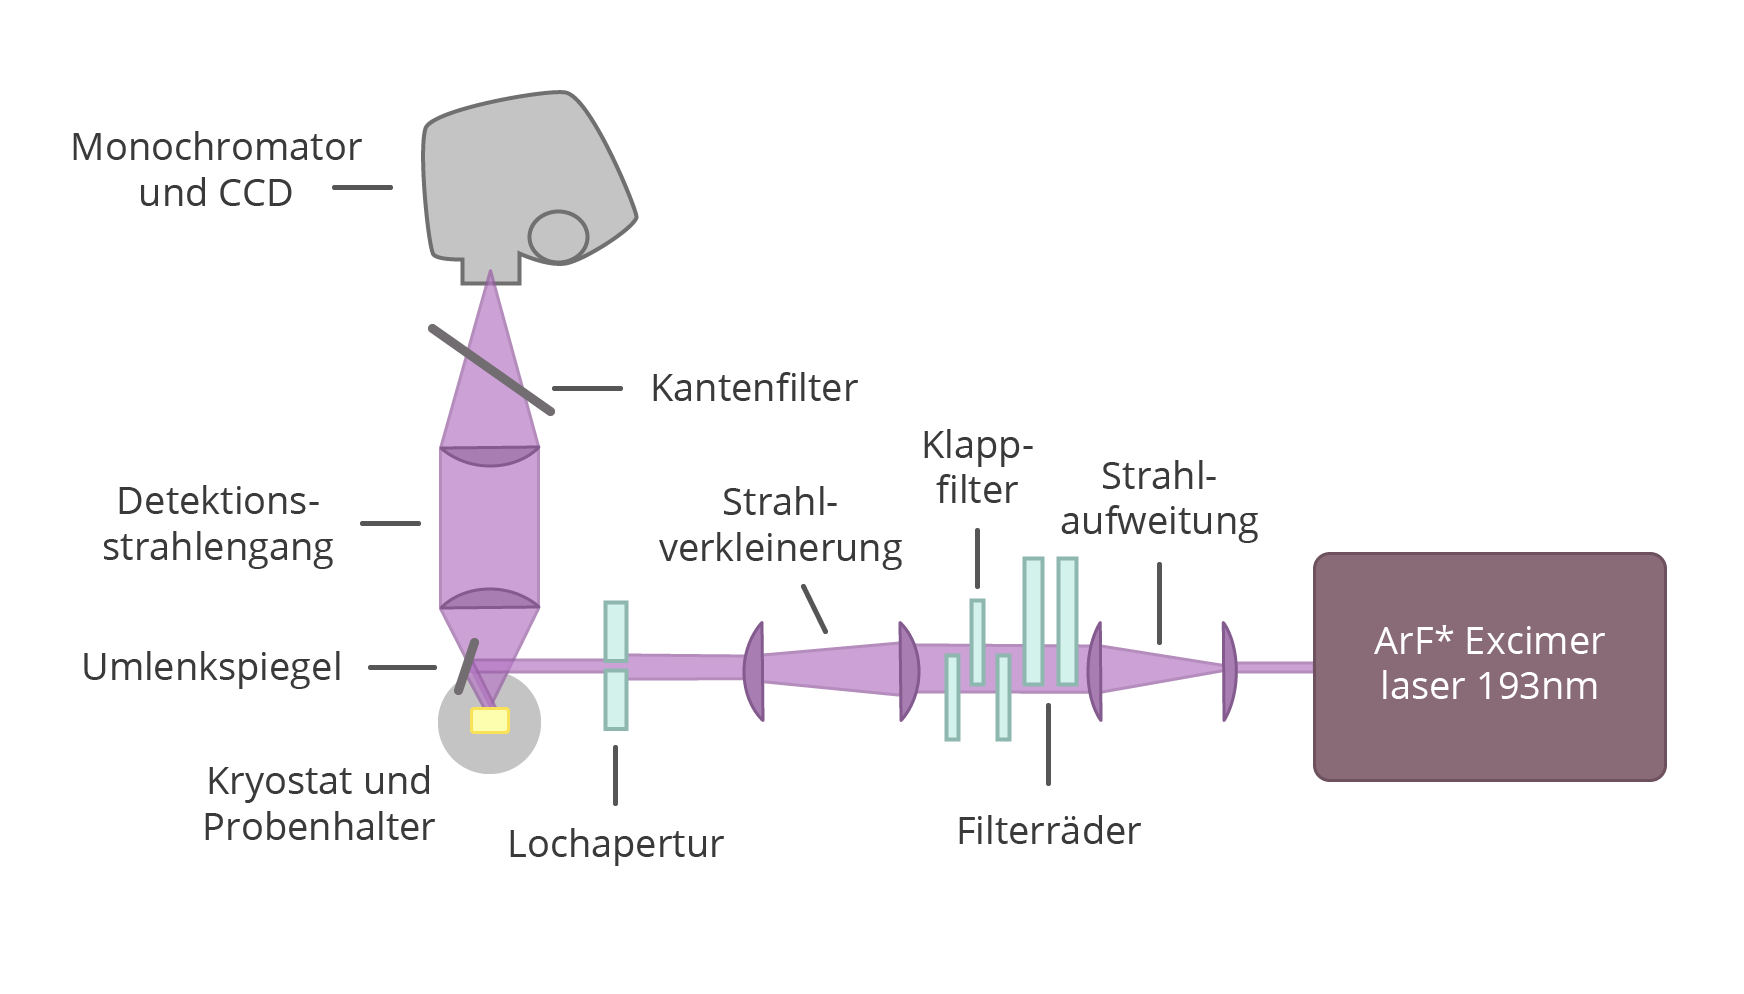
\includegraphics[width=0.8\linewidth]{Bilder/aufbauPL.png}
        \caption{Aufbau des Photolumineszenzmessplatzes der AG Kneissl. }
        \label{fig:plaufbau}
    \end{minipage}% <- sonst wird hier ein Leerzeichen eingefügt
\end{figure}
\noindent
Für die experimentelle Untersuchung der UV-Photolumineszenz wurde der PL-Aufbau der AG-Kneissl, der in Abbildung \ref{fig:plaufbau} dargestellt ist, verwendet. Der PL-Aufbau wurde von Christoph Reich in der Zeit seiner Diplomarbeit aufgebaut und während seiner Promotion erweitert \cite{creich}. 
Als Anregungsquelle für die Photolumineszenz dient ein ArF-Excimerlaser mit einer Wellenlänge von $193 \ nm$ ($6,4 \ eV$). Mit dieser Wellenlänge ist er bestens geeignet für die Überbandanregung von Nitridhalbleitern. 
Des Weiteren bietet der Aufbau die Möglichkeit von temperaturabhängigen Untersuchungen von $5 \ K $ bis $300 K$. Dies ist auch die Grundlage für die Bestimmung der IQE. 
\newline
Der Laser mit dem Modellnamen "`Xantos XS"' von der Firma Coherent bietet eine maximale Emissionsenergie von $ 5 \ mJ $ und eine einstellbare Frequenz bis zu 500 Hz bei einer Pulsdauer von $5 \ ns$.
Durch interne Rückkopplung ist eine Energiestabilisierung möglich, die die Schwankung der Anregungsleistung auf 3 Prozent minimiert. 
\newline
Die Ansteuerung des kompletten Messvorgangs erfolgt durch die Messsoftware von Christoph Reich, entwickelt in der grafischen Programmiersprache "`LabView"' von Texas Instruments. Diese ermöglicht alle nötigen Einstellungen an Pumpen, Heizern, Laser, Filtern und Spektrometer, um einen nahezu komplett automatisierten Messvorgang zu starten. Spektren können so mit verschiedenen Parametern wie Position, Anregungsleistungsdichte, Temperatur, Energiebereich und Integrationszeit aufgenommen werden und auch ein Gaswechsel ist möglich.
\newline
Beginnend vom Laser wird im ersten Schritt der Laserstrahl durch ein Linsensystem, bestehend aus einer Zerstreuungs- und Sammellinse, aufgeweitet. Dieser Schritt ermöglicht es, die Anregungsleistungsdichte zu verringern, um die am Aufbau beteiligten Geräten, insbesondere die Filterräder, nicht mit zu hohen Leistungen zu beschädigen. Mit Hilfe der Filterräder ist es möglich, die Anregungsleistungsdichte 61 stufig zu variieren und somit leistungsdichteabhängige IQE Messungen zu machen. Als nächstes passiert der Strahl ein Linsensystem aus zwei Sammellinsen für eine Strahlverkleinerung. Vor dem Auftreffen des Strahles am Probenhalter im Kryostaten passiert der Strahl noch eine Lochblende. Sie dient der Entfernung achsennaher Strahlen und um bei Bedarf den Strahldurchmesser noch weiter zu verringern. 
\newline
Um den Strahl in Richtung des Probenhalters durch das Fenster im Kryostaten zu lenken, wird ein Spiegel mit einer dielektrischen Beschichtung benutzt. Der Laserstrahl durchdringt die Fenster des Kryostaten, welche speziell für eine hohe Transmission in diesem Wellenlängenbereich ausgelegt sind. Der Kryostat selbst ist horizontal und vertikal verschiebbar, um die Messung mehrerer Proben im Probenhalter in einem Messvorgang bei gleichen Bedingungen zu ermöglichen. Die Proben werden mit einem Kleber auf dem Probenhalter selbst befestigt, bevor dieser in den Kryostaten geschoben wird. 
Die Anregung der Proben mit dem Laserstrahl führt zur probenspezifischen Emission von Licht. Diese wird von einer Linse im Strahlengang vor dem Detektor eingefangen und von einer zweiten Linse auf den Monochromatorspalt fokussiert.
\newline
Bei dem Monochromator handelt es sich um einen "`iHR 320"' des Herstellers "`Horiba"'. Zur Verfügung stehen drei Blazegitter mit $300 \thinspace \frac{Linien}{mm}$,
$600 \thinspace \frac{Linien}{mm}$ und $1800 \thinspace \frac{Linien}{mm}$. Bei der verwendeten Spaltbreite von $100 \thinspace \mu m$ entspricht die maximale Auflösung in etwa $5 \thinspace meV$ ($0,17 \thinspace nm$). Für Messungen oberhalb von $225 \thinspace nm$ besteht die Möglichkeit einen Kantenfilter in den Strahlengang einzubringen, mit dem das Laserstreulicht und dessen höhere Ordnungen aus dem Spektrum entfernt werden können. Bei dem CCD Chip handelt es sich um das Modell "`Syncerity"' von "`Horiba"' der "`open electrode"' -Bauart mit 1024x256 einzelnen Pixeln. 

\section{Messaufbau Lichtpolarisation}
\begin{figure}[!htb]
    \centering
    \begin{minipage}[t]{\linewidth}
        \centering
        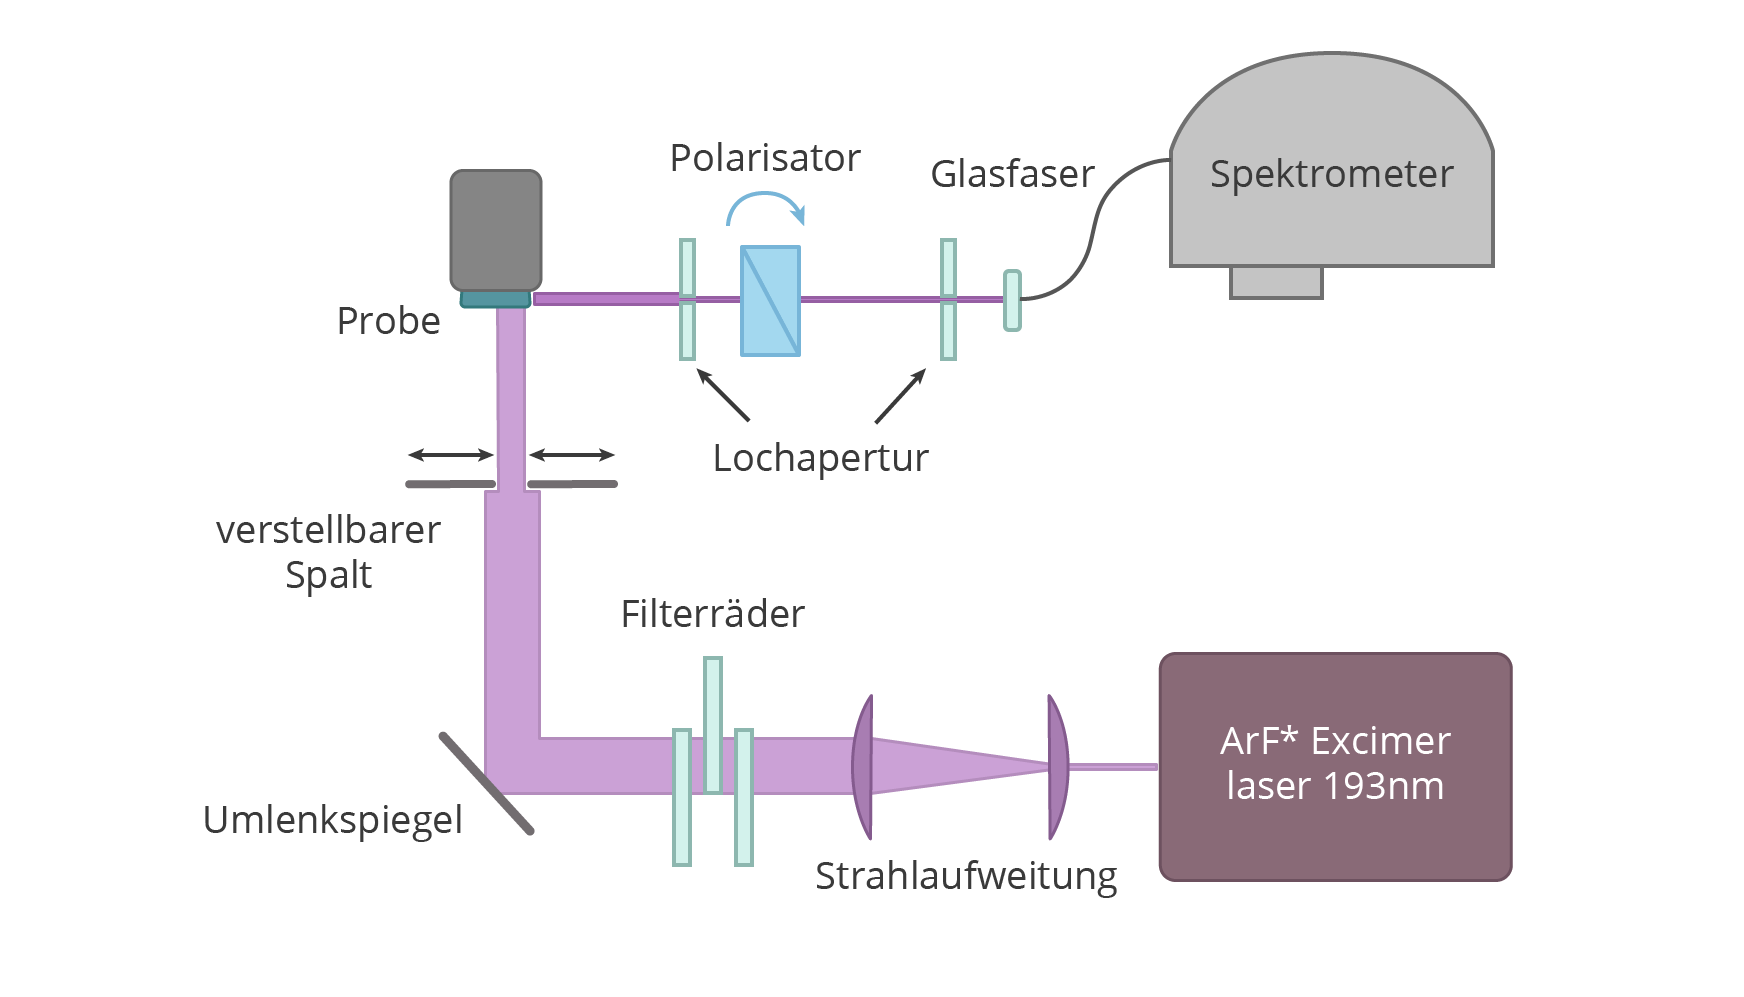
\includegraphics[width=0.8\linewidth]{Bilder/aufbauPol.png}
        \caption{Aufbau des Photolumineszenzmessplatzes der AG Kneissl zur Bestimmung der Polarisation. }
        \label{fig:polaufbau}
    \end{minipage}% <- sonst wird hier ein Leerzeichen eingefügt
\end{figure}
\vspace{1cm}
\noindent
Der Messaufbau zur Bestimmung der Lichtpolarisation ist in Abbildung \ref{fig:polaufbau} dargestellt.
Die Anregung der untersuchten Proben erfolgt senkrecht zur Probenoberfläche. Die Lumineszenz der Probe wird aus der Kante gemessen, weil TM-polarisiertes Licht nur vertikal zur c-Achse, wie in Abbildung \ref{fig:martintetm} sichtbar, emittiert wird. Die Lumineszenz wird dann unter kleinem Öffnungswinkel über eine Linse mit sich dahinter befindlicher Blende eingesammelt und parallelisiert. Das parallelisierte Licht wird dann durch einen Glan-Taylor-Polarisator geleitet. Dass das Licht parallelisiert ist, ist wegen der anisotropen Brechzahl des Polarisators wichtig. Diese ist neben der Polarisationsrichtung auch von dem Eintrittswinkel abhängig und entscheidet ob der Strahl transmittiert oder reflektiert wird \cite{0950-7671-25-12-304}. In Abhängigkeit der Orientierung des Polarisators wird TE- oder TM-polarisiertes Licht transmittiert. Der eingestellte Winkel lässt sich $1^\circ$ granular einstellen. 


	\chapter{Ergebnisse}
\thispagestyle{fancy}
\section{Untersuchung optisch gepumpter Laserstrukturen auf unterschiedlichen Templates}


Dieses Kapitel widmet sich der Untersuchung der beiden Probenreihen TS4045 und TS4048 von optisch gepumpten Laserstrukturen die aus Rezepten aus zwei unterschiedlichen Serien stammen. Die beiden Serien unterscheiden sich im wesentlichen dadurch, dass sie mit(TS4048) und ohne Übergitter(TS4045) gewachsen wurden. Jede Reihe für sich weist  zusätzlich noch Unterschiede den Proben selbst auf, so sind zwei Proben der Reihe TS4045 auf AlN-Bulk zweier unterschiedlicher Hersteller (HexaTech, IKZ) gewachsen und alle  anderen Proben auf ELO AlN/Sapphire mit jeweils 3 unterschiedlichen "offcut"-Winkeln. Tabellerisch sieht die  Zusammenstellung wie folgt aus: 

\vspace{1cm}


\setlength{\arrayrulewidth}{0.5mm}
\setlength{\tabcolsep}{0.5pt}
\renewcommand{\arraystretch}{1.5}
 

\begin{tabular}{ |c|c|c|c|c|c|   }
\hline
\multicolumn{3}{|c|}{TS4045} & \multicolumn{3}{c|}{TS4048}  \\
\hline
Endung & offcut& Template & Endung & offcut& Template \\
\hline
-2V* & 0.1$^\circ$m & ELO & -2V* & 0.1$^\circ$m & ELO \\
-2H & 0.1$^\circ$m & ELO & -2H & 0.1$^\circ$m & ELO \\
-2Z & 0.2$^\circ$m & ELO & -1 & 0.1$^\circ$m & ELO \\
-1 & 0.1$^\circ$m & Bulk(IKZ) & -2V* & 0.1$^\circ$m & ELO \\
-3* & 0.1$^\circ$m & Bulk(Hexatech) & -2V* & 0.1$^\circ$m & ELO \\
\hline



\end{tabular}




	\bibliography{Bibliographie}
\end{document}	


\begin{comment}
	\begin{figure}[b!]
    		
\includegraphics[width=0.2\textwidth]{Bilder/TU-Berlin-Logo.pdf}
    		\label{fig:tulogo}
    	\end{figure}	
\end{comment}	
